% !TEX root = ../main.tex
\section{Methods}
\label{sec:methods}

\subsection{Layer 1: flood exposure}

Each unit-week carries the CHIRPS and IMERG rain of that week and its lags, the upstream-mean rain routed down the river network and weighted by discharge, the storm exposure (whether the unit lies inside a gale swath that week), the share of people in a NOAH hazard zone (25- and 5-year return periods, missing where there is no map) and, for the four backtest storms, the new-flood share seen by Sentinel-1 (Section~\ref{sec:flood}). The Sentinel-1 feature starts in the week that contains landfall plus \sOneAfterDays{} days, the end of its after-image window, so no forecast origin sees radar from its own future.

\subsection{Layer 2: lead-lag outbreak graph}

The series is $\log(1 + \text{incidence})$, differenced over 52 weeks to remove the season and standardised inside the training window. PCMCI+, a causal discovery algorithm for time series \parencite{runge2019, runge2020}, runs with partial-correlation tests at lags 1 to \tauMax{} weeks and $\alpha_{\text{PC}} = \pcAlpha$; a lagged link between two provinces is kept when its false discovery rate (FDR) q-value is below \fdrQ{} \parencite{benjamini1995}. On pure-noise checks PCMCI+ without this step returned many false links. PageRank on the reversed graph scores sentinel provinces \parencite{page1999}, Louvain finds communities \parencite{blondel2008}, and lagged cross-correlation with the same FDR filter is the baseline graph.

\subsection{Forecast and surge probability}

One pooled XGBoost model \parencite{chen2016} per horizon (\horizons{} weeks) is trained with a multi-quantile objective at the \nQuantiles{} quantile levels of the FluSight challenge of the United States Centers for Disease Control and Prevention, on $\log(1 + \text{incidence})$, and back-transformed to cases. The features are lagged incidence, the same week of the previous year, the week of the year, rain and river lags, storm exposure, NOAH hazard, Sentinel-1 flood and leader signals from the graph; Shapley additive explanations (SHAP) give the drivers shown on the dashboard \parencite{lundberg2017}. A direct four-week model gives $R$, the probability of exceeding the unit's \surgePctl{} percentile of four-week incidence in the training window. $R$ is then recalibrated by isotonic regression \parencite{zadrozny2002}, fitted only on earlier rolling-origin forecasts whose outcome was known at the origin, and only once \calMinRows{} such outcomes exist.

\textbf{Benchmarks} are scored on exactly the same rows: Chronos-2 \parencite{ansari2025} and TabPFN-TS \parencite{hoo2025} zero-shot, each origin's forecast made from that unit's own past only; a message-passing graph network with a long short-term memory (MPNN-LSTM) \parencite{panagopoulos2021} trained on the same \refitWeeks{}-week rolling refits; and the element-wise median of the \nQuantiles{} quantiles of XGBoost and the three (the ensemble).

\subsection{Evaluation protocol}

\textbf{Rolling origin, never a random split} (Figure~\ref{fig:rolling}). From January 2018 to December 2019 the model, the graph and the surge thresholds are refit every \refitWeeks{} weeks (\nRefits{} refits) on data up to the refit date, and every origin until the next refit is forecast from them. The scores are the WIS on case counts \parencite{bracher2021}, the relative WIS against a seasonal-naive forecast (the same week of the previous year, with its empirical quantiles), the 50\% and 90\% interval coverage, and an online conformal 90\% band built from past errors only \parencite{gibbs2021}.

\begin{figure}[htbp]
\centering
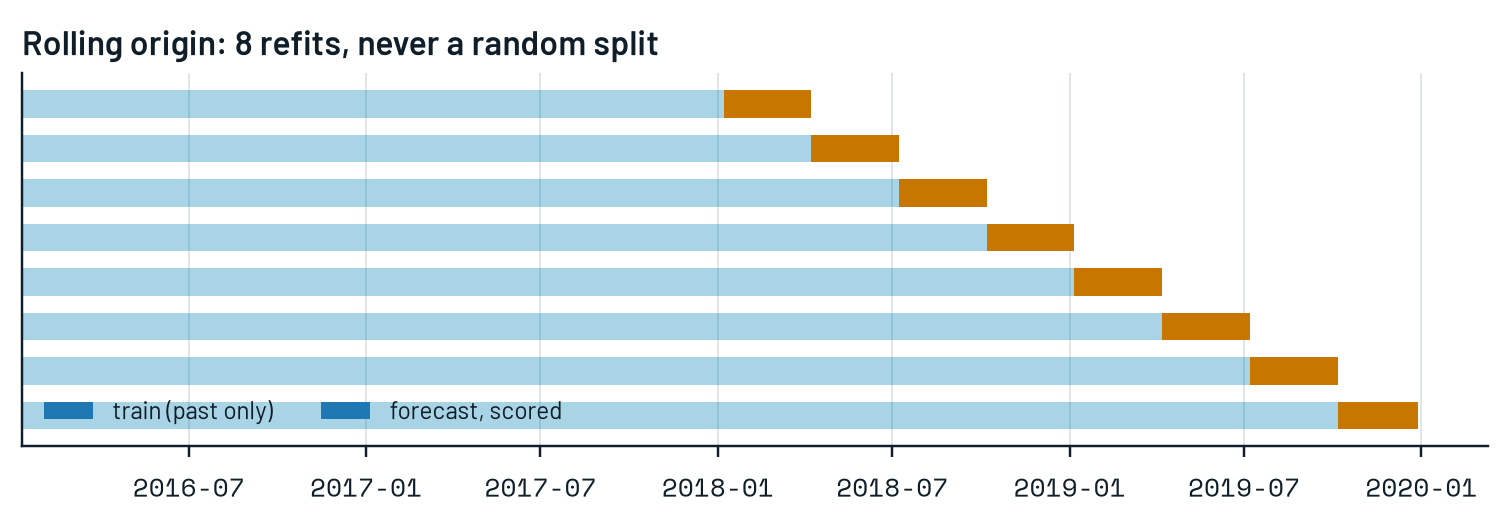
\includegraphics[width=\linewidth]{f14_rolling}
\caption{Rolling-origin evaluation: each block is forecast only from a model trained on the data before it.}
\label{fig:rolling}
\end{figure}

\subsection{Layer 3: access, two methods}

\textbf{Network.} OSM highways become a graph of junctions; roll-on/roll-off (RoRo) ferry routes are extra edges (crossing time plus half the headway); hospitals are the Humanitarian OpenStreetMap Team (HOT) health facilities plus NOAH name-matched facilities (\nHosp{}). WorldPop is summed to 1~km cells, each joined to the nearest road node, and a multi-source Dijkstra search gives the hours to the nearest hospital.

\textbf{Raster.} A cost-distance search from the same hospitals runs over the motorised friction surface of the Malaria Atlas Project (MAP) \parencite{weiss2020}, with the sea impassable except along the same ferry lines.

\textbf{Storms} apply the same rules to both methods: ferries crossing the gale swath are cancelled; roads (or cells) in observed flood (Sentinel-1, observed tracks) or in NOAH high hazard inside the swath (shifted tracks) are cut, and medium hazard slows them. A cell is cut off if it loses its route, or if its trip grows at least \cutRatio{}-fold and by more than \cutExtraH{}~h \parencite[after][]{petricola2022}. The network gives $A$, $P$ and the action tier; the per-unit minimum and maximum of the two methods give the ranges $A_{\text{lo}}$--$A_{\text{hi}}$ and $P_{\text{lo}}$--$P_{\text{hi}}$. Under-5 and 60+ people come from the High Resolution Settlement Layer (HRSL) \parencite{tiecke2017}, summed to the same cells; a cell's vulnerable people are cut off when the cell is.
